\documentclass[11pt, a4paper]{article}

\usepackage[a4paper,bindingoffset=0.2in,%
left=1in,right=1in,top=1in,bottom=1in,%
footskip=.25in]{geometry}

\usepackage[utf8]{inputenc}
\usepackage{hyperref}
\usepackage{graphicx}
\usepackage[font=small,labelfont=bf]{caption}
\usepackage{listings}
\usepackage{color}
\usepackage{caption}
\usepackage{float}
\usepackage{mwe}

\newfloat{program}{thp}{lop}
\floatname{program}{Python source code}

\newcommand{\fullref}[1]{\hyperref[#1]{\ref*{#1}:\ \nameref*{#1}}}

%Python code
\DeclareFixedFont{\ttb}{T1}{txtt}{bx}{n}{10} % for bold
\DeclareFixedFont{\ttm}{T1}{txtt}{m}{n}{10}  % for normal

\definecolor{deepblue}{rgb}{0,0,0.5}
\definecolor{deepred}{rgb}{0.6,0,0}
\definecolor{deepgreen}{rgb}{0,0.5,0}

% Python style for highlighting
\newcommand\pythonstyle{\lstset{
		language=Python,
		basicstyle=\ttm,
		otherkeywords={self},             % Add keywords here
		keywordstyle=\ttb\color{deepgreen},
		emph={loadimg},          % Custom highlighting
		emphstyle=\ttb\color{deepblue},    % Custom highlighting style
		stringstyle=\color{deepred},
		frame=tb,                         % Any extra options here
		showstringspaces=false            % 
}}

% Python environment
\lstnewenvironment{python}[1][]
{
	\pythonstyle
	\lstset{#1}
}
{}

% Python for external files
\newcommand\pythonexternal[2][]{{
		\pythonstyle
		\lstinputlisting[#1]{#2}}}

% Python for inline
\newcommand\pythoninline[1]{{\pythonstyle\lstinline!#1!}}

%opening
\title{Flowers Recognition}
\author{R\'emi Ang\\\href{https://www.udacity.com}{Udacity.com} - Machine Learning Engineering Nano Degree}

\begin{document}

\maketitle	

\section{Definition}

\subsection{Project Overview}

Object recognition is a major discipline in the field of computer vision and finds countless applications in domains asvaried as self-driving vehicles (i.e. vehicle environment detection), medicine (i.e. skin cancer diagnosis) or turism (i.e. points of interests recognition).

This project focus on the recognition of flower species with the objective to demonstrate the possibility to identify a flower variety based on a simple picture. Possible application of automatic flower recognition could be:

\begin{itemize}
	\item population acking and preservation (imagine drones taking a census of flowers in your neighbourhood)
	\item crop and food supply managment 
	\item toxicity detection ()
	\item Education (i.e. smartphone app for hitch-hiker and nature lovers)
	\item ...
	
\end{itemize}

\subsection{Problem Statement}



\subsection{metrics}

\subsubsection{Accuracy}
\begin{center}
	$accuracy = \frac{number \ of \ correct \ predictions}{total \ number \ of \ prediction} \cdot 100$ \\
\end{center}

\subsubsection{Multi-class Log Loss (cross entropy)}

\section{Analysis}

\subsection{Data Exploration and Visualization}
\label{subsec:Data_exploration_and_visualization}

The pictures have been automatically scraped from the online picture portals Flickr, Google Images and Yandex Images.

They represent single or multiple flowers under various angles, zoom, brightness conditions, life cycle stages, etc. 
\begin{center}
	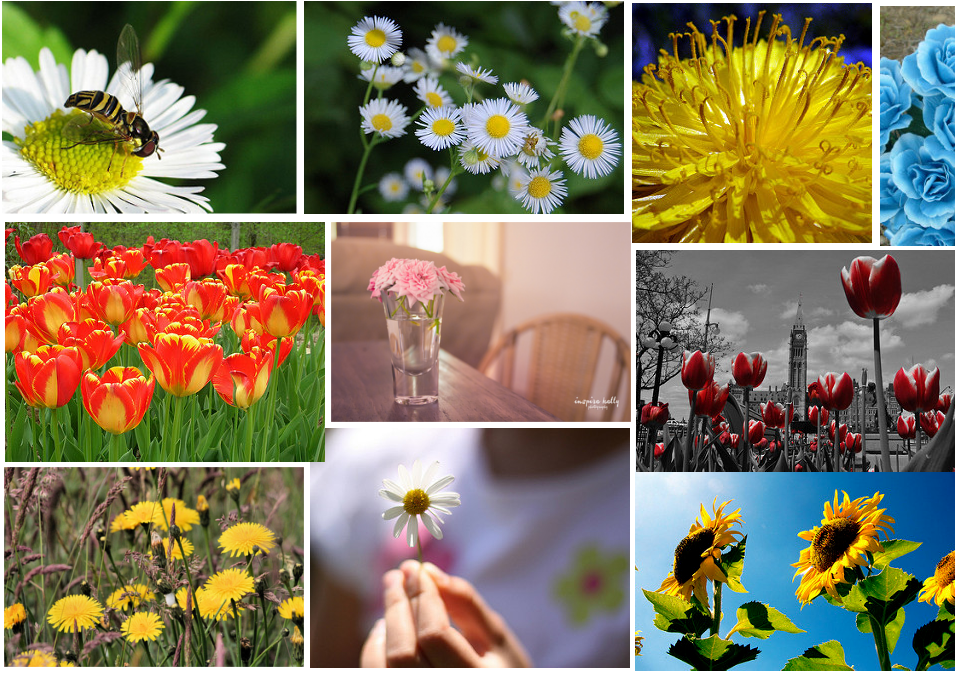
\includegraphics[scale=.25]{./sections/02_analysis/flowers_patchwork.png}
	\captionof{figure}{samples pictures}
\end{center}

The complete set of pictures distribution is as in Fig. \ref{fig:all-images-distribution}:

\begin{flushleft}
	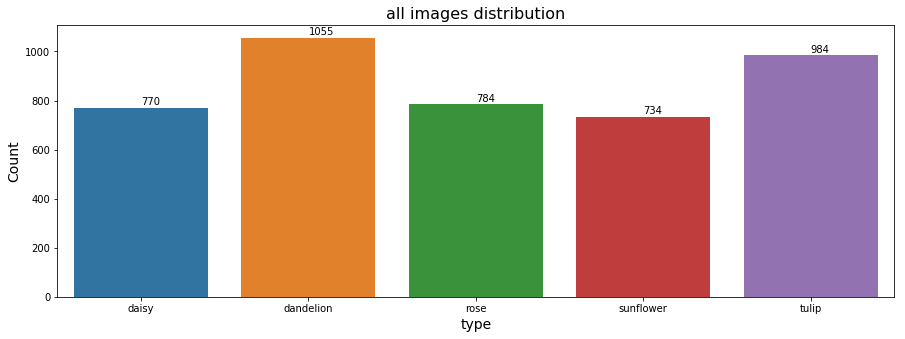
\includegraphics[scale=.5]{./sections/02_analysis/all_images_distribution}
	\captionof{figure}{All images distribution by label}
	\label{fig:all-images-distribution}
\end{flushleft}

We observe that the classes distribution is slightly unbalanced. There is an average of 865 pictures per classes to train the model, which is reasonably enough. The \textit{dandelion} class is the most represented with 1055 pictures. However, this flower variety has the particularity to be represented in 2 radically distinct state: the yellow flowers and the white "blow balls".
For this particular case, it is beneficial to have more sample to expect the model to be able to recognize both \textit{dandelion}'s aspects.  

Nevertheless, a significant number of pictures contains other subjects (persons, insects, other flowers, vase) or seem to be miss-classified. Such pictures can potentially impact negatively the model learning. A more detailed approach of the samples selection is described in chapter \fullref{subsec:Data_Preprocessing} 

\subsection{Algorithms and Techniques}

\subsubsection{pictures selection and split }

As already mentioned in the previous chapter, a large number of pictures seems inappropriate to train a model. A "blacklisting" approach will be put in place to discard them from the dataset.

On top of that, the selected pictures will be randomly split into three distinct training, validation and testing datasets. The random splitting is made in a stratified fashion in order to preserve the initial classes distribution in each set.

\subsubsection{image augmentation}

Image augmentation techniques will be used to enrich the training and validation sets. 

\subsubsection{Deep Convolutional Neural Network and transfer learning}

A deep CNN has to be trained to recognize flowers variety from pictures. Rather than designing and training a full new CNN, we will take advantage of existing reference models by applying transfer learning. The weights of all convolutional layers of the base model will be loaded and frozen as-is. The top layers will be replaced by some of our own in order to specialize the mode to flowers types recognition. 

An important part of this project will be dedicated to determine the most suitable base model to use.

\subsection{Benchmark}

The benchmark for this project is the "Flowers Species Recognition" work from Yuning Chai, Victor Lempitsky and Andrew Zisserman from the University of Oxford in 2011 \cite{Chai_BiCos, Chai_BiCos_demo} . 

This two-steps approach consist of the segmentation of the pictures and the training of a kernelized SVM classifier. The best model reach a prediction accuracy of 80.0\% and is able to recognize flowers among 102 different variety.

The goal of this project is to reach at least this accuracy, however only 5 flower species are considered. 



\section{Methodology}

\subsection{Data Preprocessing}
\label{subsec:Data_Preprocessing}

\subsubsection{Pictures scan}

\subsubsection{Sample blacklist}

As already mentioned in \fullref{subsec:Data_exploration_and_visualization}, a significant amount of pictures in the dataset are likely to negatively impact the learning of the mode. Our flower recognition model is intended to be used in an application where the images are supposed be focused on one or few flowers of the same type, from a close to middle-range distance (1 to 10 meters), in natural colours.

The black-listing of pictures aim to discard samples:
\begin{itemize}
	\setlength\itemsep{1pt}
	\setlength{\parskip}{0pt}
	\setlength{\parsep}{0pt}
	\item which don't have a ".jpg" extension (some python web scrapping routine can be found in the \textit{dandelion} subfolder)
	\item not representing a flower
	\item wrongly classified
	\item containing other subjects (persons, insects, objects,...)
	\item close ups
	\item wide shots with fields, mountains, landscapes...
	\item drawings
	\item with artistic filters significantly denaturing the original colour
\end{itemize}

After the manual visualization of all samples, the blacklist contains 1059 items (24.5\% of the total dataset) stored in a text file (\texttt{blacklist.txt}). The data loading implementation read this file and discards any file found in the list. 

\begin{center}
	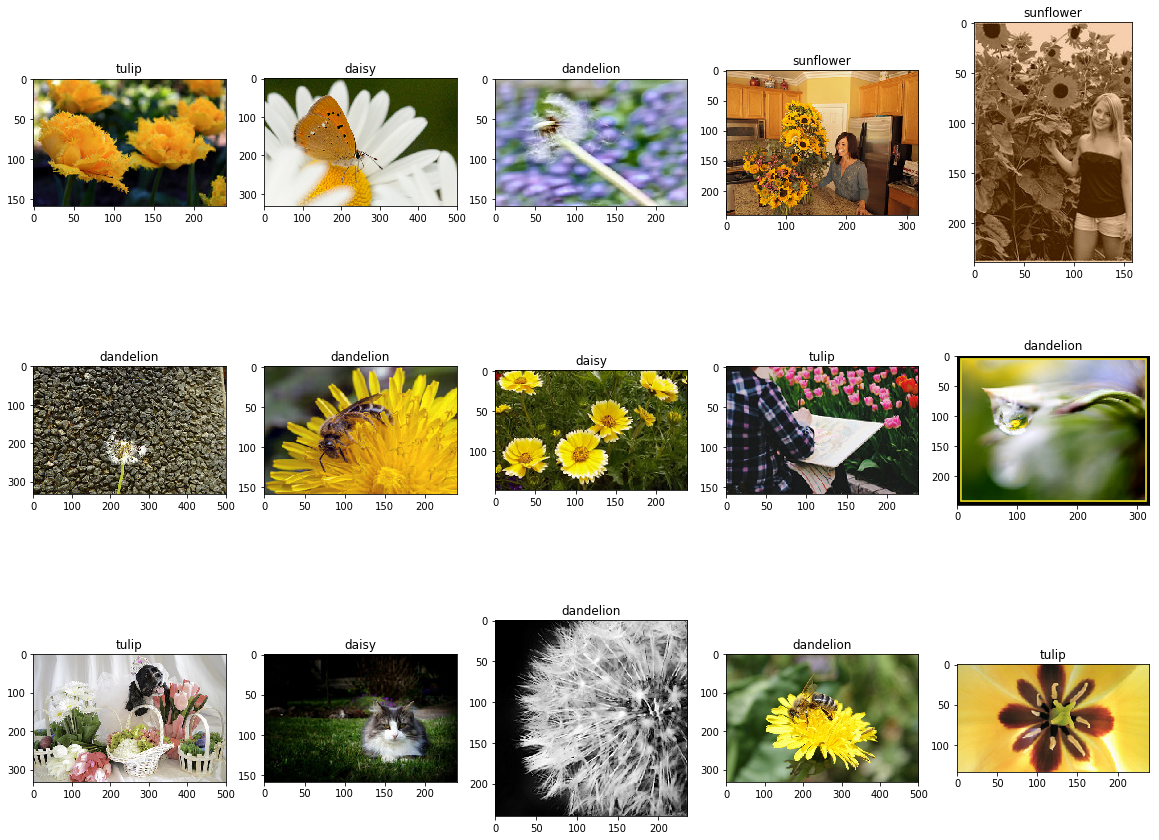
\includegraphics[scale=.35]{./sections/03_methodology/output_11_1.png}
	\captionof{figure}{samples of black listed pictures}
\end{center}

\captionof{program}{picture file scan and filtering}
\begin{python}
from sklearn.datasets import load_files 
	
path = "./flowers"

blacklist_file = "blacklist.txt" # list of files to be removed drm the dataset

#read blacklist
with open(blacklist_file, 'r') as f:
	blacklist = f.readlines()
blacklist = [path + s.strip() for s in blacklist]

# scan all files stored in the data folder
data = load_files(path, load_content=False)
all_flowers_files = np.array([s.replace('\\', '/') for s in data["filenames"]])

# identify blacklist indexes
isvalid_file = [True if f not in blacklist else False for f in all_flowers_files]
flowers_files = all_flowers_files[isvalid_file]

# flowers_targets = np_utils.to_categorical(data["target"],5)
flowers_targets = data["target"][isvalid_file]
flowers_target_names = data["target_names"]
\end{python}

After filtering, we observe that the  new classes distribution is comparable to the original one. The classes are ow represented by 654 samples on average:

\begin{flushleft}
	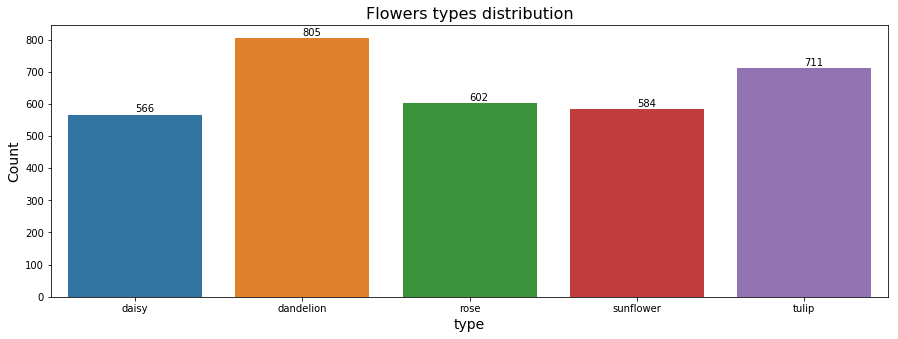
\includegraphics[scale=.5]{./sections/03_methodology/output_13_0.png}
	\captionof{figure}{Images distribution after blacklist filtering}
\end{flushleft}

\newpage
\subsubsection{Training, validation and testing split}

The dataset is randomly split in 3 parts using the \texttt{train\_test\_split} from \texttt{sklearn.model\_selection} package, using the \texttt{stratify} option in order to preserve the original classes distribution in each split:

\begin{itemize}
	\setlength\itemsep{1pt}
	\setlength{\parskip}{0pt}
	\setlength{\parsep}{0pt}
	\item Training (76.5\% - 2500 samples)
	\item Validation (8.5\% - 278 samples)
	\item Testing (15\% - 491 samples)
\end{itemize}

\captionof{program}{picture files train/valid/test split}
\begin{python}
from sklearn.model_selection import train_test_split	
	
# train+valid / test split
test_size = .1

flowers_files_train_valid, flowers_files_test, flowers_targets_train_valid, flowers_targets_test = train_test_split(
flowers_files, flowers_targets, 
test_size = test_size, 
stratify=flowers_targets)

# train / valid split
valid_size = .2
flowers_files_train, flowers_files_valid, flowers_targets_train, flowers_targets_valid = train_test_split(
flowers_files_train_valid, flowers_targets_train_valid, 
test_size = valid_size, 
stratify=flowers_targets_train_valid)
\end{python}

\begin{flushleft}
	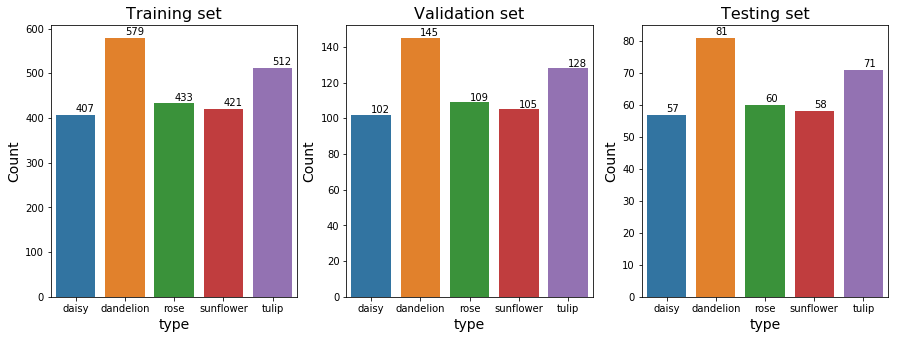
\includegraphics[scale=.5]{./sections/03_methodology/output_18_0.png}
	\captionof{figure}{Stratified images distributions after train/valid/test split}
\end{flushleft}

\newpage
\subsubsection{Dataset loading in memory}

The images are loaded in RBG colors and resized in a 299x299 shape using OpenCV "\texttt{cv2}" python package. 
Targets labels are one-hot-encoded using the \texttt{to\_categorical} method from the \texttt{keras.utils.np\_utils} package.

\captionof{program}{Image loading with openCV}
\begin{python}
from keras.utils import np_utils
from tqdm import tqdm
import cv2

def loadimg(path):
	"""
	load and resize an image
	return a (299, 299, 3) array
	"""
	img = cv2.imread(path)
	img_r = cv2.resize(img, (299, 299))
	return img_r

x_train = np.array([loadimg(f) for f in tqdm(flowers_files_train)]).reshape(-1, 299, 299, 3)
y_train =  np_utils.to_categorical(flowers_targets_train)

x_valid = np.array([loadimg(f) for f in tqdm(flowers_files_valid)]).reshape(-1, 299, 299, 3)
y_valid =  np_utils.to_categorical(flowers_targets_valid)

x_test = np.array([loadimg(f) for f in tqdm(flowers_files_test)]).reshape(-1, 299, 299, 3)
y_test =  np_utils.to_categorical(flowers_targets_test)

\end{python}

\newpage
\subsubsection{Image augmentation}
\label{subsubsec:Image_augmentation}

In order to enrich the dataset, image augmentation is applied to the training and validation datasets using the \texttt{ImageDataGenerator} utility from the \texttt{keras.preprocessing.image} package. This step is also used to normalize the features: all values are divided by 255. 
No image augmentation is applied on the testing set which is meant to represent real case images for the model evaluation. 

\captionof{program}{Augmented image generators}
\begin{python}
	from keras.preprocessing.image import ImageDataGenerator
	train_datagen = ImageDataGenerator(
	rescale=1./255,
	shear_range=0.2,
	zoom_range=0.2,
	horizontal_flip=True)
\end{python}

\begin{center}
	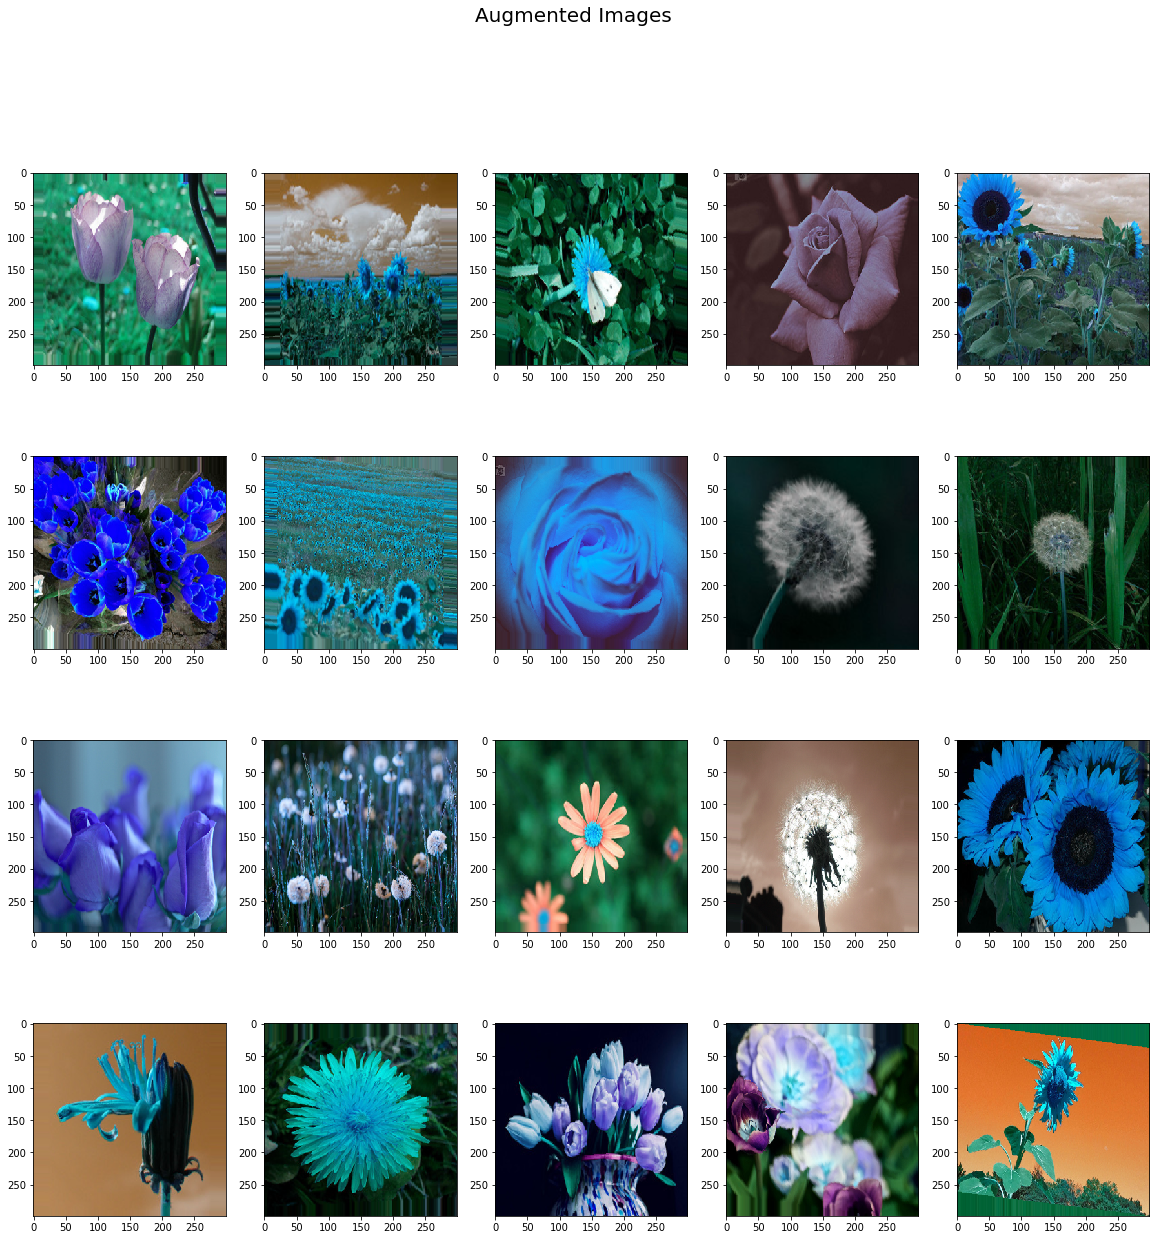
\includegraphics[scale=.3]{./sections/03_methodology/output_26_0.png}
	\captionof{figure}{samples of augmented training images}
\end{center}

\subsection{Model Implementation}

\subsubsection{CNN architecture}
The targeted CNN architecture is the combination of a fixed weights base model and custom top layers specialized in the prediction of flower varieties.

The flower recognition CNN final architecture has been implemented as following:

\begin{itemize}
	\setlength\itemsep{1pt}
	\setlength{\parskip}{0pt}
	\setlength{\parsep}{0pt}
	\item Base model
	\item Flatten layer
	\item Dense layer, 500 units, ReLu activation
	\item Dropout layer, 0.3 drop probability
	\item Output layer: Dense layer, 5 units, Softmax activation
	\item Optimizer: Adam with learning rate $\alpha=1e^-3$ and decay $d=1e^-6$ 
	\item loss function: categorical cross-entropy
	\item metrics : accuracy
\end{itemize}

\captionof{program}{construction of a CNN with VGG16 as base model}
\begin{python}
from keras.applications.vgg16 import VGG16
from keras.layers import Flatten, Dense, Dropout
from keras.models import Model
from keras.optimizers import Adam

# load the base model, do not include top layers
base_model = VGG16(weights='imagenet', include_top=False, input_shape=(299,299,3))  

# freeze the layers of the base model
for layer in base_model.layers:
	layer.trainable = False   

# top layers:
x = Flatten()(base_model.output)
x = Dense(500, activation='relu', name='fc1')(x)
x = Dropout(0.3)(x)
x = Dense(5, activation='softmax', name='fc2')(x)

model = Model(inputs=base_model.input, outputs=x)

# set up the optimizer
opt = Adam(lr = 1e-3, decay=1e-6)

# compile the model
model.compile(loss = 'categorical_crossentropy', optimizer=opt, metrics=['accuracy'])
\end{python}

This architecture is inspired by the solution proposed by A. Akashnian in his "Flowers are mesmerizing" notebook published on \href{https://www.kaggle.com/aakashnain/flowers-are-mesmerizing}{Kaggle.com}  \cite{NAIN_notebook}.

\subsubsection{CNN training}

The model is trained with the augmented pictures generator specified in \fullref{subsubsec:Image_augmentation},  on 50 epochs with batches of 32 samples (= 73 steps/epoch). The model weights are saved via a \texttt{ModelCheckpoint} each time that the validation loss each a new minima. The training historic is stored in order to later analyse the accuracies and losses evolution during the training. In order to speed-up the processing time, the model has been trained on an Amazon Web Services GPU instance (50 to 60 seconds per epochs).

\captionof{program}{model training}
\begin{python}
from keras.callbacks import ModelCheckpoint 
	
batch_size = 32
epochs = 50
saved_models_dir = 'saved_models'

#if it doesn't exist, create the saved model directory 
if not os.path.isdir(saved_models_dir):
	os.mkdir(saved_models_dir)

# define the model weight h5 storage
best_weights_h5 = os.path.join(saved_models_dir,
	'weights.best.flowers_recognition.{}.hdf5'.format(base_model_name))

# model checkpointer
checkpointer = ModelCheckpoint(filepath=best_weights_h5, 
	verbose=1, save_best_only=True)

# training
training_hist = model.fit_generator(train_datagen.flow(x_train, y_train, batch_size=batch_size),
	steps_per_epoch=x_train.shape[0] // batch_size,
	epochs=epochs, 
	verbose=1, 
	callbacks=[checkpointer],
	validation_data=valid_datagen.flow(x_valid, y_valid, batch_size=batch_size),
	validation_steps=x_valid.shape[0] // batch_size)
	
\end{python}

\subsection{Model Refinement}

\subsubsection{Base Model selection}

The \texttt{keras.applications} package offers some pre-trained models. In frame of this project, the VGG16, VGG19 and Resnet50 based models have been individually tested on 10 epochs. 

%--- VGG16 based model
\begin{center}
	\centering
	\begin{minipage}{0.5\textwidth}
		\centering
		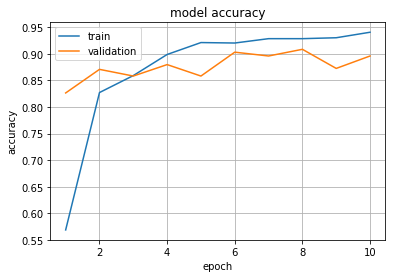
\includegraphics[width=0.9\textwidth]{./sections/03_methodology/VGG16_10epochs_acc.png}
		\captionof{figure}{VGG16 - 10 epochs Accuracy}
		\label{VGG16_10e_Acc}
	\end{minipage}\hfill
	\begin{minipage}{0.5\textwidth}
		\centering
		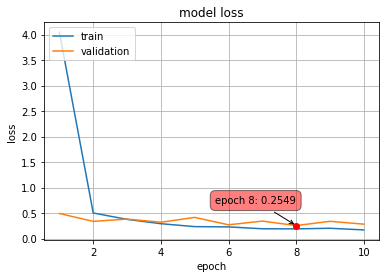
\includegraphics[width=0.9\textwidth]{./sections/03_methodology/VGG16_10epochs_loss.png} 
		\captionof{figure}{VGG16 - 10 epochs Loss}
		\label{VGG16_10e_Loss}
	\end{minipage}
\end{center}

According to Fig. \ref{VGG16_10e_Acc} and \ref{VGG16_10e_Loss}, VGG16 based model seems to learn extremely fast after the first back-propagation at epoch 1. It then constantly improves during the next epochs. After 10 epochs, the best validation loss achieved is 0.2549  and the accuracy 0.91 at epoch 8. This base model seems to be a good candidate for our flowers classifier.

--- VGG19
\begin{center}
	\centering
	\begin{minipage}{0.5\textwidth}
		\centering
		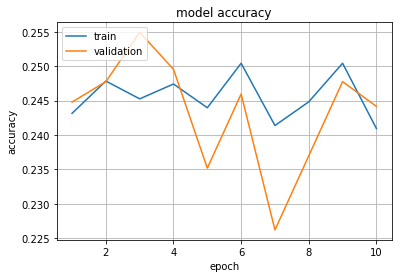
\includegraphics[width=0.9\textwidth]{./sections/03_methodology/VGG19_10epochs_acc.png}
		\captionof{figure}{VGG19 - 10 epochs Accuracy}
		\label{VGG19_10e_Acc}
	\end{minipage}\hfill
	\begin{minipage}{0.5\textwidth}
		\centering
		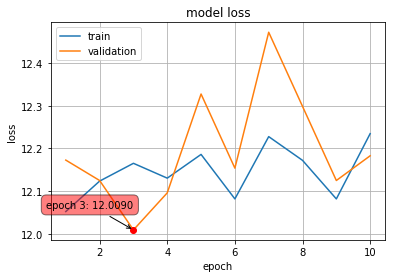
\includegraphics[width=0.9\textwidth]{./sections/03_methodology/VGG19_10epochs_loss.png} 
		\captionof{figure}{VGG19 - 10 epochs Loss}
		\label{VGG19_10e_Loss}
	\end{minipage}
\end{center}

According to Fig. \ref{VGG19_10e_Acc} and \ref{VGG19_10e_Loss}, the VGG19 based model doesn't seem able to learn. The average training accuracy of 24\% is comparable to random guesses performance. This base model will not be considered for the flower classifier.

%---Resnet50
\begin{center}
	\centering
	\begin{minipage}{0.5\textwidth}
		\centering
		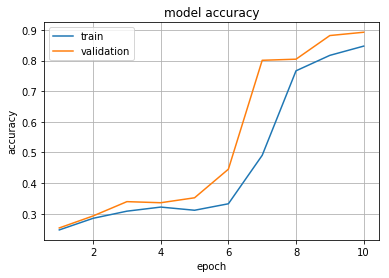
\includegraphics[width=0.9\textwidth]{./sections/03_methodology/Resnet50_10epochs_acc.png}
		\captionof{figure}{Resnet50 - 10 epochs Accuracy}
		\label{resnet50_10e_Acc}
	\end{minipage}\hfill
	\begin{minipage}{0.5\textwidth}
		\centering
		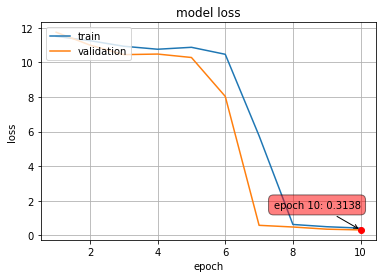
\includegraphics[width=0.9\textwidth]{./sections/03_methodology/Resnet50_10epochs_loss.png} 
		\captionof{figure}{Resnet50 - 10 epochs Loss}
		\label{resnet50_10e_Loss}
	\end{minipage}
\end{center}

According to Fig. \ref{resnet50_10e_Acc} and \ref{resnet50_10e_Loss}, it takes up to 7 epochs for this model to achieve reasonably good performances. It reach its best validation loss at the 10th epoch with 0.3138 and an accuracy of nearly 90\%, letting suggest that it could even more improve with longer training. 
\\\\
\textbf{\underline{base model selection - conclusion:}}

The best performing flower classifier on 10 epochs is the \textbf{VGG16 based model}. Therefore, it has been selected to perform a full training on 50 epochs.


\newpage
\section{Results}

The VGG16 based flower classifier is trained on 50 epochs (about 45 minutes on GPU instance). According to Fig. \ref{VGG16_50e_Acc} and \ref{VGG16_50e_Loss}, the model achieve the best validation loss at epoch 33 with 0.2122. The validation accuracy stagnate at 90\% after the 10th epoch.

\begin{center}
	\centering
	\begin{minipage}{0.5\textwidth}
		\centering
		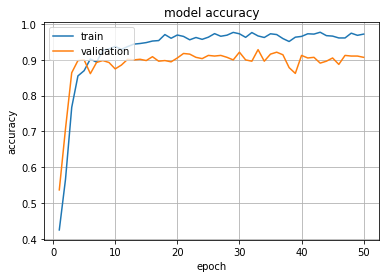
\includegraphics[width=0.9\textwidth]{./sections/04_results/output_33_0.png}
		\captionof{figure}{VGG16 - 50 epochs Accuracy}
		\label{VGG16_50e_Acc}
	\end{minipage}\hfill
	\begin{minipage}{0.5\textwidth}
		\centering
		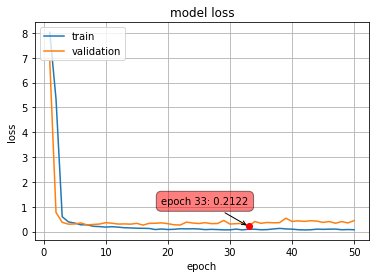
\includegraphics[width=0.9\textwidth]{./sections/04_results/output_33_1.png} 
		\captionof{figure}{VGG16 - 50 epochs Loss}
		\label{VGG16_50e_Loss}
	\end{minipage}
\end{center}

\subsection{Model Accuracy}

The model accuracy is compute by loading the best loss weights, scaling the test set and evaluating the model with its \texttt{evaluate} method on the scaled test dataset:
\\
The VGG16 based flower classifier achieve an accuracy of \textbf{89.30\%} on the testing set.

\captionof{program}{best weights loading and evaluation of the model accuracy}
\begin{python}
base_model_name = 'VGG16'
best_weights_h5 = 'saved_models/weights.best.flowers_recognition.{}.hdf5'.format(base_model_name)

# load best loss weights
model.load_weights(best_weights_h5)	

# scale test dataset
xtest_scaled = x_test.astype('float32')/255

# evaluate model accuracy
score = model.evaluate(xtest_scaled , y_test, verbose=1)

# display accuracy in stdout
print('\nTest accuracy: {:.2f}%'.format(score[1] * 100))
\end{python}

\subsection{Justification}

The predictions are evaluated for each sample of the test dataset:

\captionof{program}{test pictures prediction}

\begin{python}
import numpy as np

predictions = np.array([np.argmax(model.predict(np.expand_dims(x, axis=0))) \
	for x in tqdm(xtest_scaled)])
\end{python}

The confusion matrix displayed in Fig. \ref{fig:output402} confirms the good performance of the model.

\begin{itemize}
	\item 80.7 \% of the test \textit{daisies} are correctly classified. The type of flower is mostly confused by the model by \textit{dandelions}.
	\item 92.6 \% of the test \textit{dandelions} are correctly classified. This type of flower is mostly confused by the model with \textit{sunflowers}. This remarquable score demonstrate that the model is able to identify the \textit{dandelions} both in yellows flower state and white "blow-balls" (see discussion in Chapter  \fullref{subsec:Data_exploration_and_visualization}). 
	\item 85.0 \% of the test \textit{roses} are correctly classified. This type of flower is mostly confused by the model with \textit{tulips}.
	\item 94.8 \% of the test \textit{sunflowers} are correctly classified. This the most accurately predicted type of flower. 
	\item 91.5 \% of the test \textit{tulips} are correctly classified. This type of flower is mostly confused by the model with \textit{roses}.
\end{itemize}

\begin{center}
	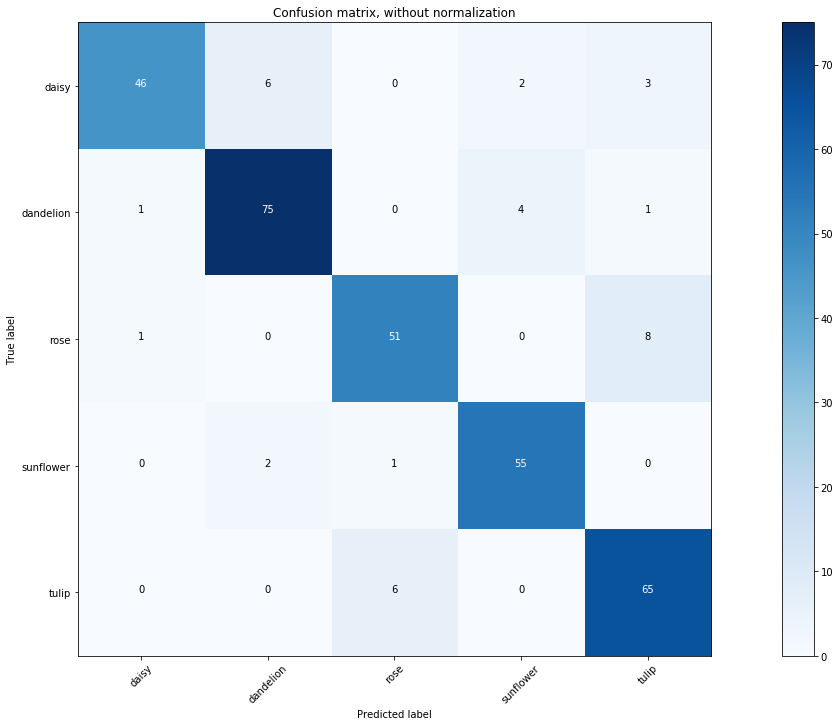
\includegraphics[scale=.4]{sections/04_results/output_40_2}
	\captionof{figure}{test pictures predictions - confusion matrix}
	\label{fig:output402}
\end{center}









\section{Conclusion}

\subsection{Free-Form Visualization}

\subsubsection{Test samples prediction}

A sample of successful tests predictions is displayed in Fig. \ref{fig:output420} with the predicted label and the true label shown in the title. 

\begin{center}
	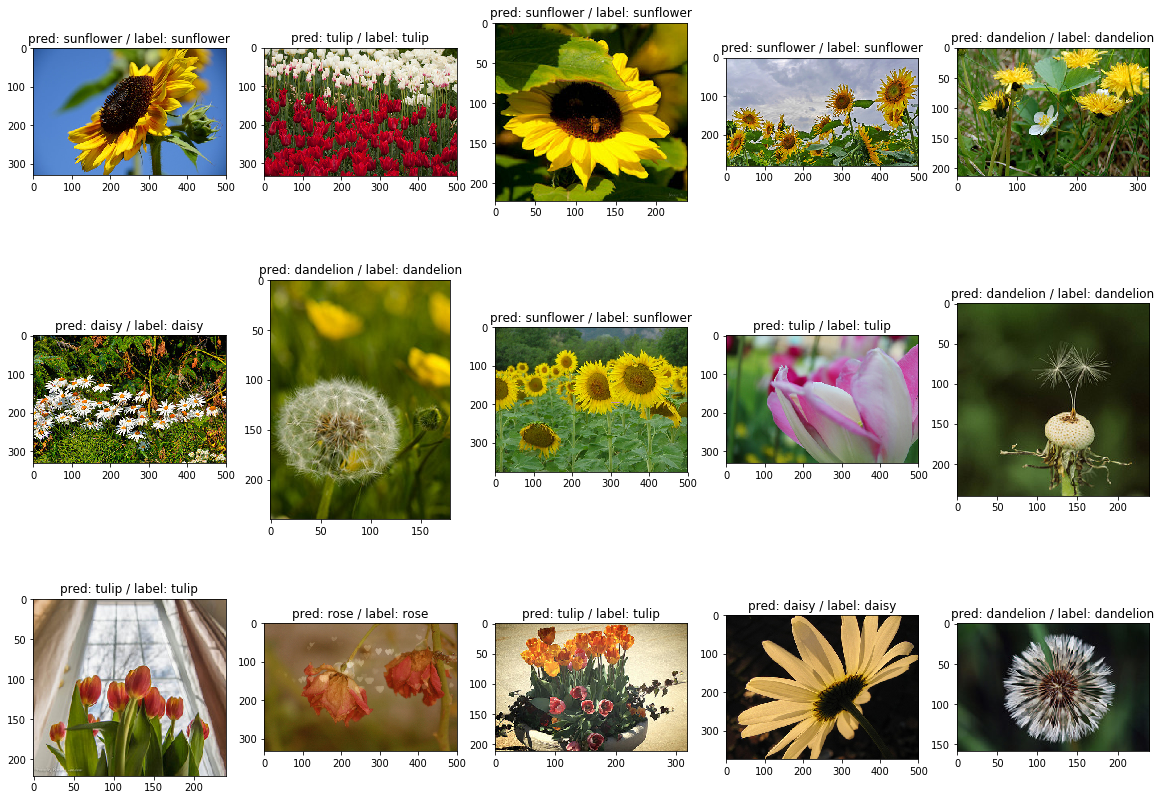
\includegraphics[scale=.35]{sections/05_conclusion/output_42_0}
	\captionof{figure}{Sample of test picture flower recognition}
	\label{fig:output420}
\end{center}

\subsubsection{Failed  prediction}

All the test samples that the model failed to identify correctly are display on Fig. \ref{fig:output430}.

\begin{center}
	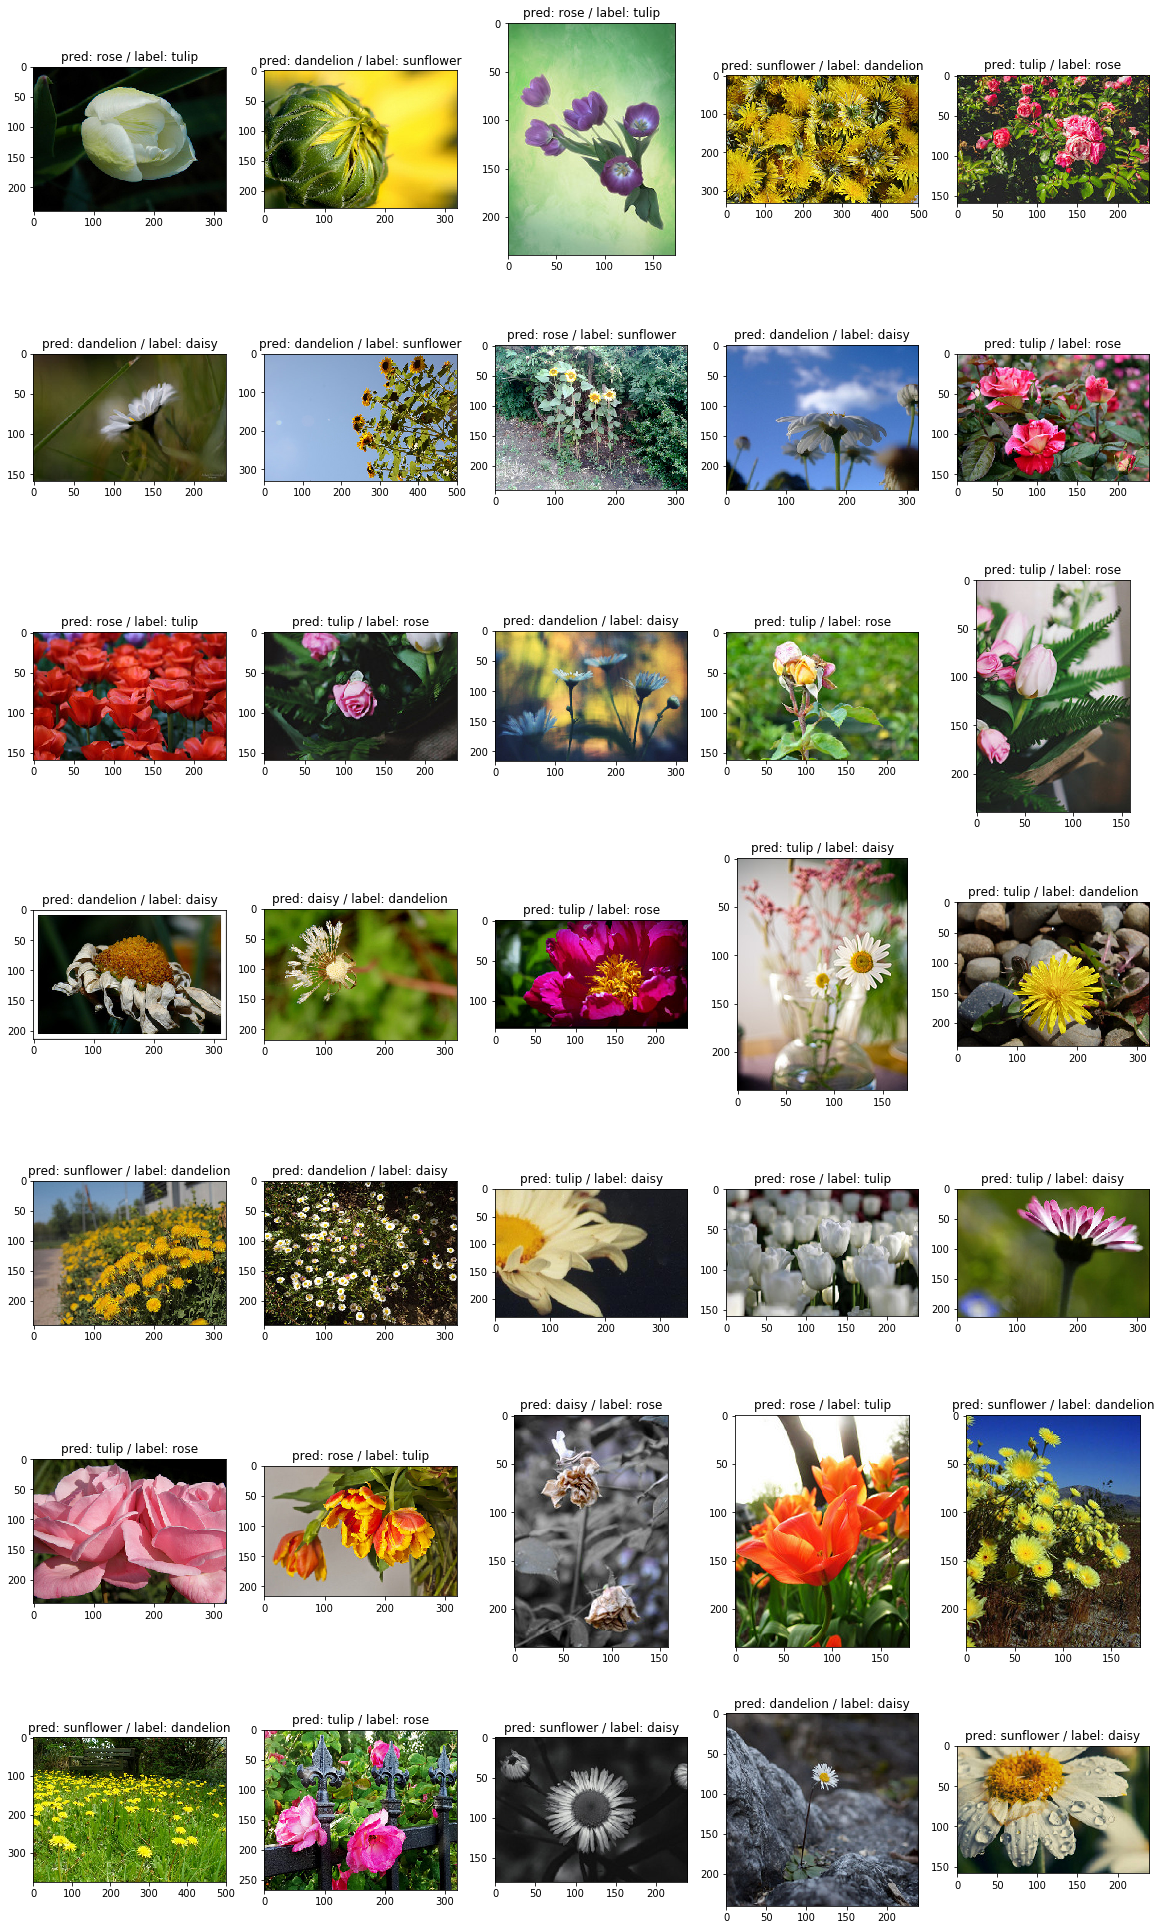
\includegraphics[scale=.35]{sections/05_conclusion/output_43_0}
	\captionof{figure}{failed predictions in the test dataset}
	\label{fig:output430}
\end{center}


\subsection{Reflection}

The process used for this project can be summarized as follow:

\begin{enumerate}
	\setlength\itemsep{1pt}
	\setlength{\parskip}{0pt}
	\setlength{\parsep}{0pt}
	\item Find a relevant/challenging problem to solve
	\item find already existing work(s) in order to set the benchmark
	\item Find a dataset suitable for answering this problem
	\item Clean up and pre-process the dataset to make it training-ready
	\item Test different base model for the CNN and select the best performing one
	\item Train the final chosen CNN in the cloud
	\item Evaluate the model and analyse the results
\end{enumerate}

One particular difficult and tedious task has been the manual selection of samples to keep or remove from the dataset. This work is hardly automatable and had to be performed case by case, based on arbitrary rules and intuition. 

I have been positively surprised by the differences in performance between the three based models tested. According to the references, VGG16 is the model among the three having the lowest accuracy on the ImageNet validation dataset \cite{Keras_applications}. However, this exercise comforted me in necessity to try different approaches.  

\subsection{Improvement}

The main improvement for this project would be to increase the amount of flower classes. It would be particularly interesting to train the same CNN on the 100+ flowers types used by the BiCos-SVM model \cite{Chai_BiCos_demo}.
It would also worth trying other base models that have not been considered in this study.
It would be beneficial to deeper analyse prediction failure cases in order to identify failures root cause and adapt accordingly the dataset or the model if feasible.
Finally, in order to deploy the model in real life, it would be necessary to develop a mobile application able to directly process a picture taken by the device and return to the user a prediction.

\bibliographystyle{plain}
\bibliography{bibliography}

\end{document}
